\section{Experimento 1}

El primer experimento que presentamos en el trabajo fue realizado en una cafetería (Starbucks), por la tarde, mientras había aproximadamente unas 15 personas a la vista usando dispositivos móviles. La captura de paquetes duró casi una hora.

\subsection{Resultados}

Primero, la fuente S. Nuestra hipótesis sobre esta fuente, basándonos en lo que dijimos anteriormente en el trabajo, es que el símbolo de los paquetes de broadcast tendrá una información mucho mas alta que el símbolo de los paquetes unicast.

\begin{figure}[H]
  \centering
  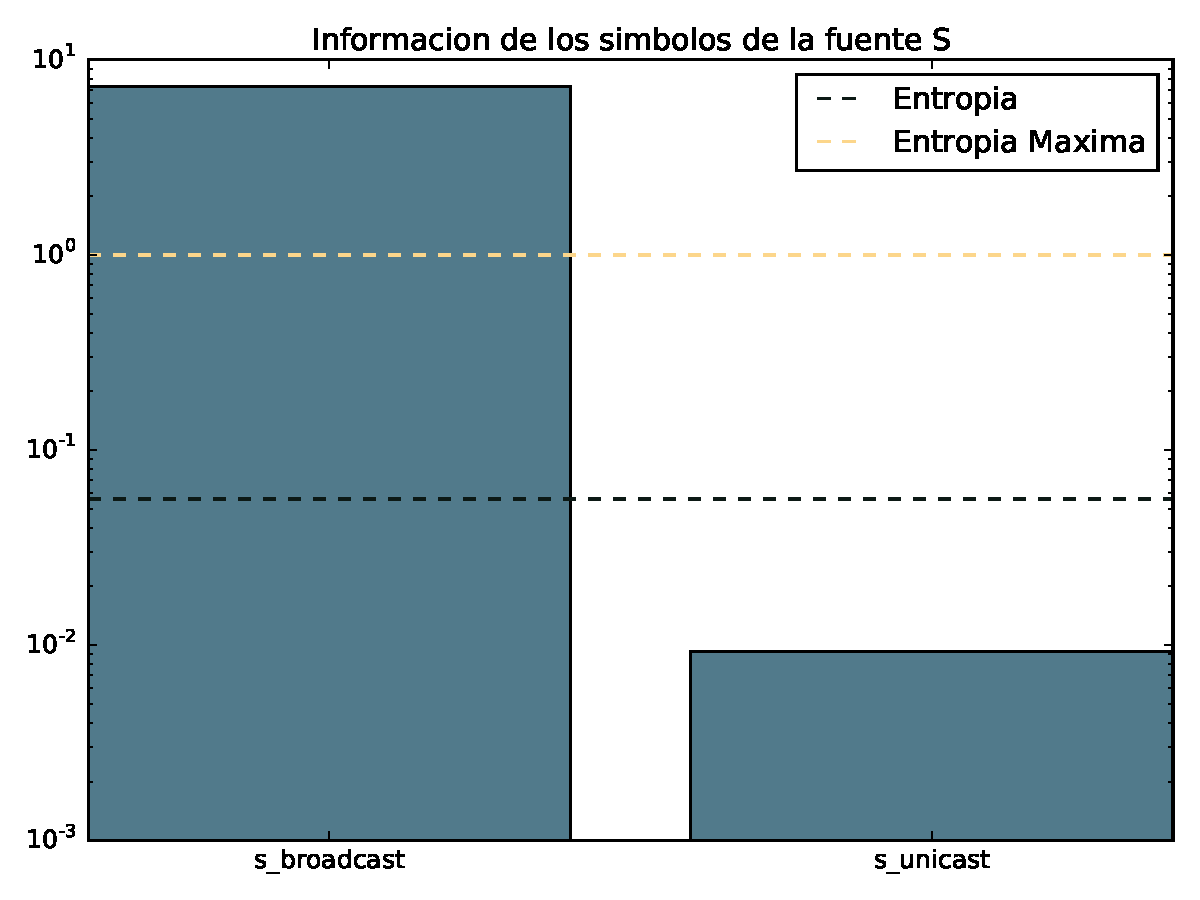
\includegraphics[width=8.5cm]{exp_starbucks/grafico1.pdf}
  \caption{\normalfont }
\end{figure}

Nuestra hipótesis sobre la red es que habrá unos pocos dispositivos que se conectaran a un router, y quizás si el router y el AP ambos tienen IPs dentro de la red, aparezcan como dispositivos separados en la red.
Analizaremos esto, y todas nuestras otras hipótesis en al discusión.

\begin{figure}[H]
  \centering
  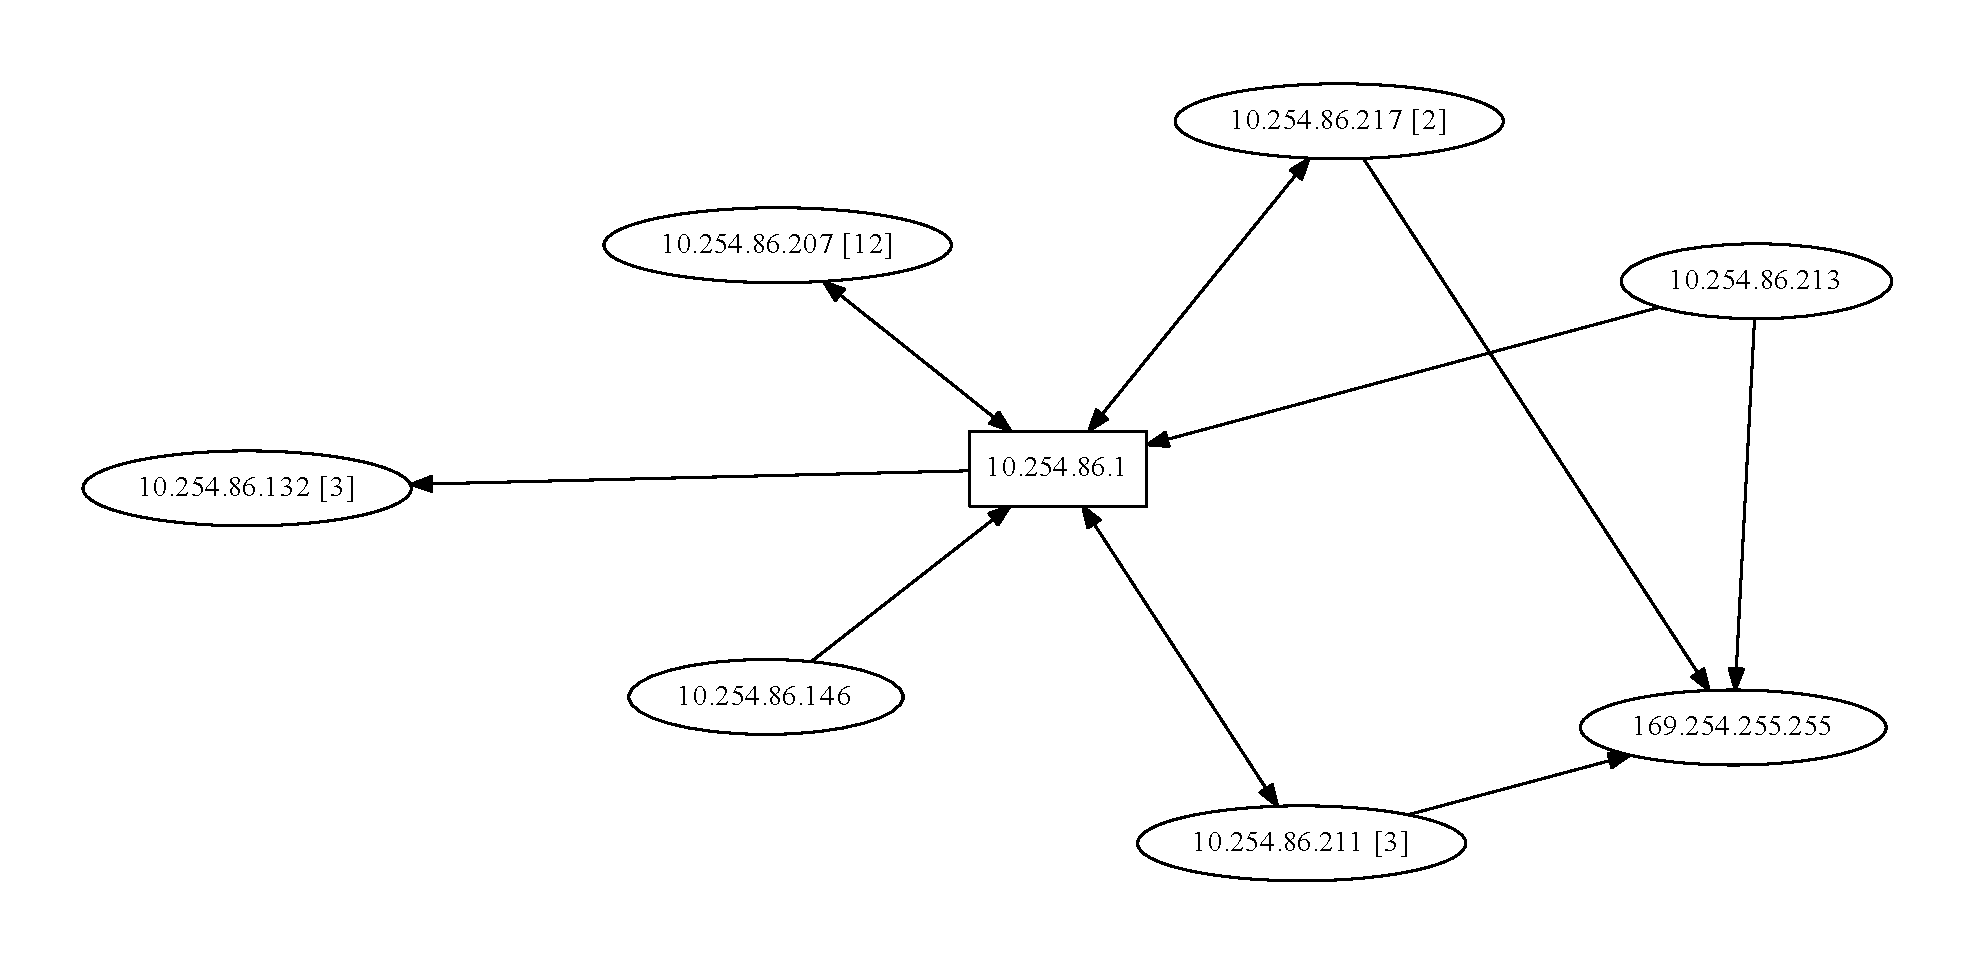
\includegraphics[width=8.5cm]{exp_starbucks/grafico2.pdf}
  \caption{  \normalfont Grafo de conectividad de la red, inferido de los paquetes who-has. Para ver con mayor detalle, se puede hacer zoom-in en el pdf. }
\end{figure}

Sobre la fuente S1, esperaremos que haya un dispositivo que tenga menor información que el resto, y esperaremos que este sea el router. Además, esperamos que el resto de los dispositivos sean hosts, y tengan menor información si son más activos en la red.

\begin{figure}[H]
  \centering
  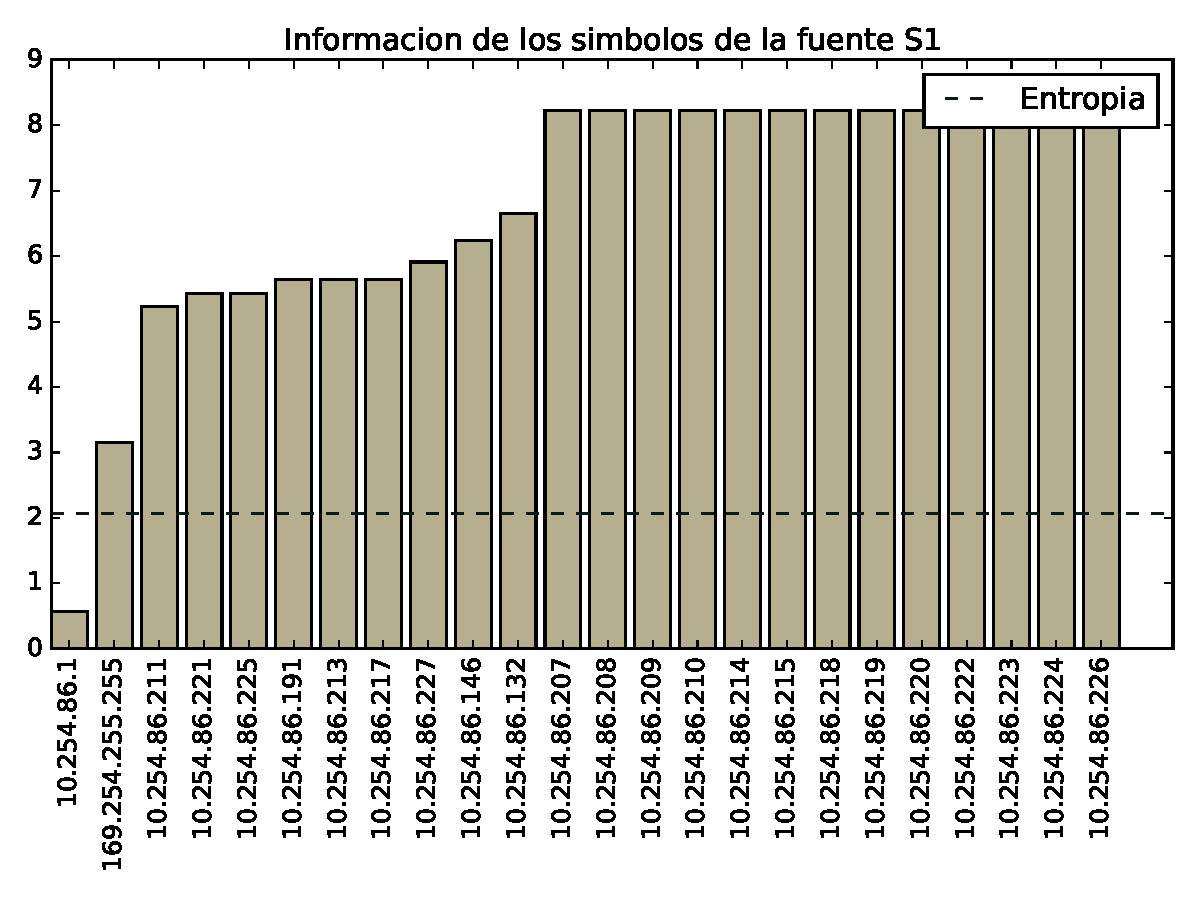
\includegraphics[width=8.5cm]{exp_starbucks/grafico3.pdf}
  \caption{ \normalfont Información de los símbolos de la fuente S1: solamente los nodos con menor información son representados.}
\end{figure}

\subsection{Discusión}

Analicemos los resultados que vimos en la sección anterior.

Empecemos por la fuente S. Como esperabamos, la información del símbolo asociado a los paquetes broadcast es muy alta. Como dijimos al principio del trabajo, asociaremos esto a dos hechos: 

\begin{enumerate}
  \item Podemos ver todo lo que pasa en la red, en particular, podemos ver todos los paquetes que se le envian a los host distintos del nuestro.
    Esto en general nos va a permitir inferir o bien que la red es una red Wi-Fi, o bien que es una red Ethernet muy simple, sin switches o subnets.
  \item Además, que la comunicación en la red es efectiva, o sea que los hosts están comunicando cosas unos con otros o bien con dispositivos fuera de la red.
    Si la mayoría de los paquetes fuera broadcast, eso nos daría la idea de que no se está dando comunicación efectiva entre los hosts, si no, que por ejemplo, todos los mensajes que se intercambian son de control.
\end{enumerate}

Por esa razón, es mucho más común en este caso que un paquete sea unicast que broadcast. Por ello, entropía de la fuente S no va a ser máxima, dado que la información de los únicos dos símboos es muy diferente.

Continuando con el análisis del grafo de la red y la fuente S1, se observa que hay 24 nodos. El nodo distinguido (según la fuente S1) es lo que parece ser el router. Inferimos que es el router porque su último octeto es 1, que es el valor default para routers. 


Las IP de los nodos corresponde a la red 10.254.86.0/24. La mayoría de los hosts terminaban en octetos distintos de 1, excepto el router, que como dijimos tenía a 1 como último octeto. Esto nos da la pauta de que efectivamente lo que estamos viendo es una red, que además se corresponde con la red Wi-Fi de la cafetería.

Nos parece razonable afirmar que el resto de los nodos son hosts conectados a la red Wi-Fi, dado que por lo que se veía en la cafetería, había un mínimo de 15 dispositivos conectados a la red, y además el resto se comporta de la misma manera. 

Notemos que los nodos que no se conectan solamente con el router (10.254.86.1), se conectan con el nodo 169.254.255.255. El nodo que tiene esta IP ss un caso que puede ser considerado anómalo o borde y fue explicado anteriormente. Es importante decir que apareció en todos los experimentos con Wi-Fi que hicimos, con lo cual es interesante tenerlo en cuenta para futuros experimentos.


La cantidad de nodos del grafo indica que los dispositivos conectados a la red Wi-Fi son los que observamos, más algunos que no pudimos ver.

Es muy interesante que la fuente propuesta y nuestro grafo de nodos nos permitió de una manera muy precisa comprender la disposición y organización de la red. En las conclusiones haremos un análisis general de este y el resto de los experimentos.






